\subsection{Filter Design}

The typical Human can only hear frequencies in the range of 20Hz through 20kHz, and this range only decreases as humans age  \cite{human:rg}.  Using the website \url{http://onlinetonegenerator.com/hearingtest.html}, we will test the hearing range of each member listening to the presentation.  When the hearing test was performed within our group, the highest audible range was 15kHz.  With this simple demonstration, the audience will understand why a low pass filter that filters frequencies above 20KHz would not impact the quality of the sound.  Understanding that humans cannot hear above and below certain thresholds creates an opportunity transmit audio signals with smaller bandwidths.  

In order to filter out higher frequencies in an audio signal transmission, we will build a low pass filter.  Specifically, we will describe how a low pass filter is created using a finite number of non-zero filter coefficients which is called a \textit{Finite Impulse Response} filter or FIR.  Given the impulse response, we can find the coefficients of the filter, and vice versa \cite{notes:class}.  For example, 

\begin{figure}[h!]
	\centering
	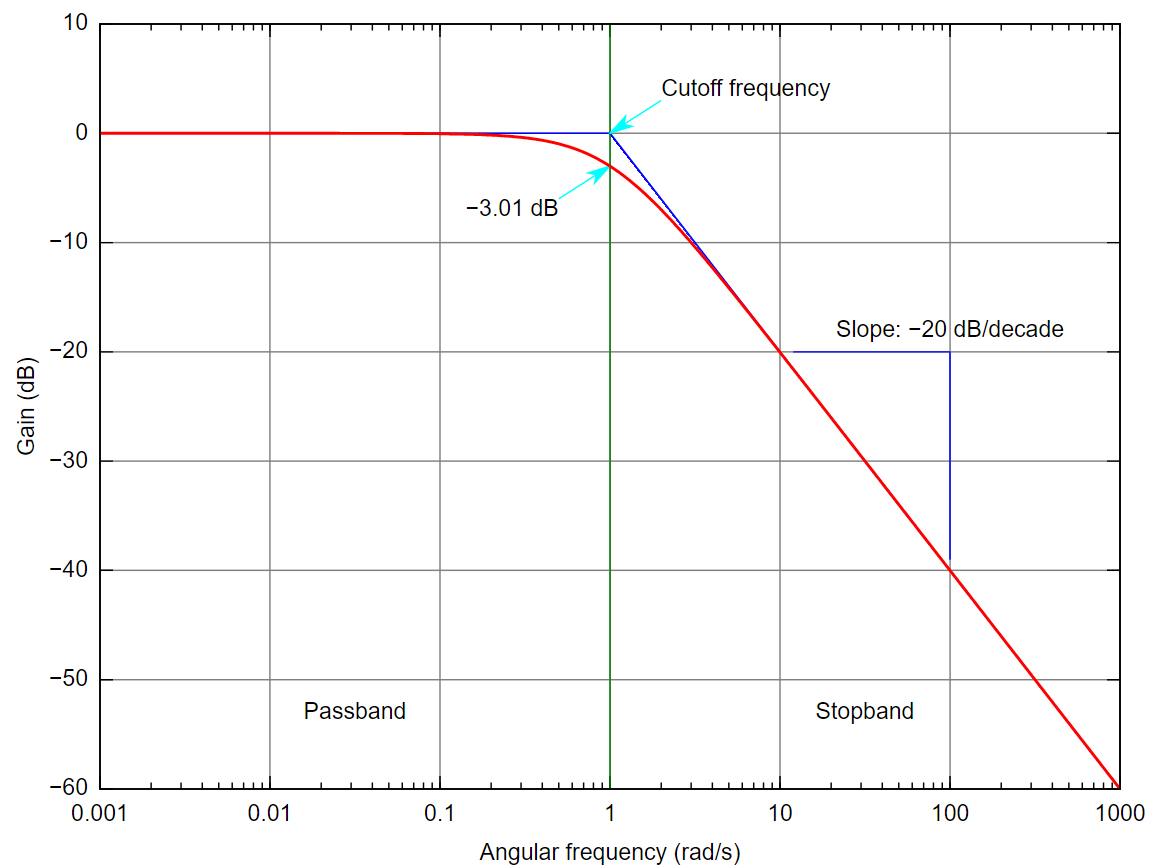
\includegraphics[scale = .5]{low_pass.png} %this is useful too \includegraphics[width = \linewidth]
	\caption{Example of Low Pass Filter: \url{https://upload.wikimedia.org/wikipedia/commons/6/60/Butterworth_response.svg}}
\end{figure}    
 
